\documentclass{school-22.211-notes}
\date{February 13, 2012}

\begin{document}
\maketitle


%%%%%%%%%%%%%%%%%%%%%%%% Neutron Slowing Down and Thermalization %%%%%%%%%%%%%%%
\lecture{Neutron Slowing Down and Thermalization}

\topic{Summary: Reuss Ch 7 Neutron Slowing Down}
\begin{enumerate}
\item Decouple absorption and scattering is possible because absorption is complicated at lower energies, whereas scattering is the opposite (b/c inelastic and anisotropic aspects). 

\item Elastic vs. inelastic: elastic scattering has no threshold, making it the most important one in neutron slowing down. Inelastic scattering has a threshold of a few MeV for light nuclei, and a few tens of keV for heavy nuclei, making it mainly observed in the fuel materials particularly \ce{^{238} U}. 

\item In Lab system, laws of elastic collision: 
  \begin{align}
    \frac{E_{nf}}{E_{ni}} &= \frac{A^2 + 1 + 2A \cos \theta}{(A+1)^2} = \frac{1}{2} \left[ 1 + \alpha + (1-\alpha) \cos \theta \right] \\
    \cos \psi &= \frac{1 + A \cos \theta}{\sqrt{A^2 + 1 + 2A \cos \theta}} \\
    \alpha &= \frac{(A-1)^2}{(A+1)^2} = \mbox{min ratio between final n energy and initial} 
  \end{align}

\item In CMCS, scattering is isotropic in solid angle $\Omega$(except very high energy), which implies that $\cos \theta$ is uniform, and $E_{nf}$ is uniform:

  \begin{align}
    P(\theta) \dtheta &= \frac{1}{2} \sin \theta \dtheta = \frac{1}{2} \derivative |\cos \theta| \\
    P(E) \dE &= \frac{\dE}{(1-\alpha) E_i} 
  \end{align} 

\item In Lab system, scattering towards the front it favored. The mean of $\cos \psi$ is $\mu = \expect{ \cos \psi} = \frac{2}{3A}$. 

\item Lethargy, a unitless measurement of energy (the idea comes from laws of elastic collision governs an energy ratio):
  \eqn{ u = \ln \frac{E_{\mathrm{ref}}}{E} }
Notice as time goes, neutrons slow down, $u$ increases, making it like a measure of the age of the neutrons. Then we know that the uniform distribution of energy becomes a decreasing exponential distribution for lethargy gain: 
\begin{align}
w &= u_f - u_i = -\ln \left[ \frac{1}{2} ( 1 + \alpha + (1-\alpha) \cos \theta ) \right] \\
w_{min} &= 0 \\
w_{max} &= \epsilon = -\ln \alpha \\
P(w) \dw &= \frac{e^{-w}}{1 - \alpha} \dw \\
\expect{w} &= \xi = 1 - \frac{\alpha \epsilon}{1 - \alpha} 
\end{align}
$\xi$ is like the efficiency of slowing down by a nucleus. That is, neutrons advance by $\xi$ lethargy units on average at each collision. Then to overcome the total lethargy interval $U = \ln \frac{E_0}{E_1}$, the number of collisions needed is:
\eqn{ n = \frac{U}{\xi} }
\begin{figure}
  \centering
  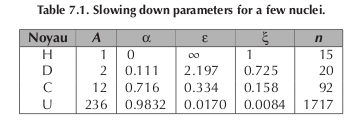
\includegraphics[width=3in]{images/slowing-down-parameter.png}
  \caption{Slowing Down parameters}
\end{figure}

\item Moderating power is the best measure of a material's ability to slow down neutrons. It has two forms:
\eqn{\mbox{per atom basis} = \xi \sigma_s \fsp \fsp \fsp \mbox{per volume basis} = \xi \Sigma_s   }
A good moderating material should have: high slowing down (hence light nuclei), low capture (D, Be, C), moderating power (take into account both high slowing down and high scattering xs). Water has the highest moderating power, but it requires an enriched fuel (around 1\%). 
\begin{figure}
  \centering
  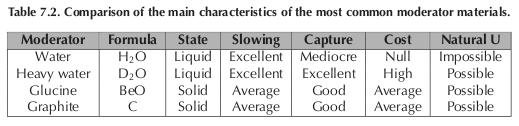
\includegraphics[width=3in]{images/moderator-comparison.png}
  \caption{Comparison of Characteristics of Moderators}
\end{figure}

\item Laws of inelastic collision. Elastic scattering is important for moderators because they are light; inelastic scattering is important for heavy materials like the fuel because they have almost no elastic collision. Minimum energy of the neutron for an inelastic collision is:
\eqn{ E_{\mathrm{threshold}} = \frac{A+1}{A} Q } 

\item Slowing down equations: a simplified Boltzmann equation performing neutron counts that depends on one variable, either velocity or energy or lethargy. We pick lethargy. Then we assume an infinite, homogeneous medium with a source uniform in space and time. 

\item First form of the slowing down equation (7.1.9):
  \begin{align}
    \rho(u) \du 
    &= \mbox{arrival density} = \begin{array}{l}
      \mbox{\# neutrons arriving per time and per volume} \\
      \mbox{in d$u$ between $u$ and $u + \du$ following a scattering to $u'$} 
      \end{array} \\
    &= \overbrace{\int_{-\infty}^u \Sigma_s (u') \Phi(u') \du'}^{\textcircled{1}} \overbrace{ P(u'\to u) \du }^{\textcircled{2}} \\
    \textcircled{1} &= \mbox{\# neutrons travelling in du' and scattered per time and per volume} \\
    \textcircled{2} &= \mbox{probability a neutron scattered at u' will be transferred in du} \\
    \rho(u) &= \int_{-\infty}^u \Sigma_s (u'\to u) \Phi(u') \du' \\
    S(u) + \rho(u) &= \boxed{S(u) + \int_{-\infty}^u \Sigma_s (u'\to u) \Phi(u') \du  = \Sigma(u) \Phi(u) }
  \end{align}
  In the specific case of COM isotropic, monatomic elastic slowing down, the transfer probability is:
  \eqn{P(u'\to u) = P(u\to u') = \frac{e^{-(u-u')}}{1-\alpha} }
\item Decay of neutron spectrum by successive scattering events (7.2.2): producing spectrum by adding up successive scattering events;
\item Slowing down without absorption (7.2.3). Asymptotic value of flux: 
  \eqn{ \Phi_{as} (u) = \frac{S}{\xi \Sigma_s(u)} }
  If we plot flux vs. lethargy, all isotopes would fluctuate (Placzek transient) before reaching the asymptotic flux value, except H which immediately reaches $\Phi_{as}$. 
\item Slowing down in hydrogen (7.2.4): uses Green's function; the Dirac distribution compensates for the source in the equation; the Heaviside step function makes sure the neutrons scattered at least once scattered beyond, not below, the original lethargy. 
\item Slowing down with resonance absorptions (which is low energy) (7.2.5): we can approximate resonance absorption of the following types
  \begin{enumerate}
    \item Black resonance trap: 
      \eqn{ 1 - p = \int_0^{\gamma} \int_{u-\epsilon}^0 \du' \frac{1}{\xi} \frac{e^{-(u-u')}}{1 - \alpha} = \frac{1 - e^{-\gamma} - \alpha \gamma}{\xi (1-\alpha)}  }
      when $\gamma$ is small, we can simplify the above to be $1 - p = \frac{\gamma}{\xi}$. 
    \item Narrow grey resonance trap:
      \eqn{ 1 - p  = \int_{\mathrm{trap}} \frac{\Sigma_a(u)}{\Sigma_t(u)} \frac{\du}{\xi} }
    \item A set of narrow grey resonance traps: we express each resonance in exponential form, and find the product of them:
      \begin{align}
        p_i &= 1 - \int_i \frac{\Sigma_a(u)}{\xi \Sigma_t (u)} \du = \exp \left[ -\int_i \frac{\Sigma_a(u)}{\xi \Sigma_t(u)} \du \right] \\
        p &= \prod_i p_i = \exp \left[ - \Sum_i \int_i \frac{\Sigma_a(u)}{\xi \Sigma_t(u)} \du \right]
      \end{align}
    \item General expression:
      Because the integrated function is zero outside of the resonance traps, we can simply write,
      \eqn{p =  \exp \left[ - \int_ \frac{\Sigma_a(u)}{\xi \Sigma_t(u)} \du \right] }
      This is the general expression for resonance escape probability. 
  \end{enumerate}
\item Slowing down with low, slowly varying absorption (which is high energy) (7.2.6). 

  \begin{enumerate}
  \item Greuling-Goertzel approximations for slow and gradually varying absorption: 
  \item Wigner approximation for resonance absorption: 
  \end{enumerate}
\end{enumerate}

%%%%%%%%%%%%%%%%%%%%%%%%%%%% Ch 9 %%%%%%%%%%%%%%%%%%%%%%%%%%%%%%%%
\topic{Summary: Reuss Ch 9 Thermalisation of Neutrons}
\begin{enumerate}
\item For monatomic gas, there is thermal agitation and no chemical bonds, we can approximaet with Maxwell distribution. 
\item For any thermaliser, the neutron spectrum at equilibrium and in the absence of absorption (or with low capture) would be a Maxwell spectrum. A Maxwell spectrum depends on $E, kT$. 
\item Microreversibility principle/detailed balance: at equilibrium and with no absorption, the number of transfers by diffusion from $\dE$ to $\dE'$ as transfers in the other direction from $\dE'$ to $\dE$. 
\item Scattering equation (9.1.4): 
\eqn{ \Sigma_s(E', E, \mu) = \Sigma_s (E') P(E' \to E) P(\mu) = C^{te} \sqrt{\frac{E}{E'}} \exp \left[\frac{E'-E}{2kT} \right] S(\alpha, \beta)  }
\item Thermalisation equation (9.1.5): 
  \eqn{ \int_0^{E_{\mathrm{cutoff}}} \Sigma_s (E') \Phi(E') \dE' P(E' \to E) + \overbrace{\int_{E_{\mathrm{cutoff}}}^{\infty} \Sigma_s(E') \Phi(E') \dE' P(E'\to E)}^{S_{\mbox{slow-down}}(E)} = \Sigma_t(E) \Phi(E) }
  and the slow-down equation, 
  \eqn{ \int_{-\infty}^{u} \Sigma_s (u') \overbrace{P(u' \to u)}^{\frac{\exp(-(u-u'))}{1 - \alpha}} \Phi(u') \du' + S(u) = \Sigma_t(u) \Phi(u) }
  The two are similar, except:
  \begin{enumerate}
  \item The slowing down equation only down scatters, whereas thermalisation equation can transfer energies in both directions. The upper boundary $E_{\mathrm{cutoff}}$ is the energy separating the thermalization domain from the slowing down domain. 
  \item The `source' in the thermalisation equation $S_{\mbox{slow-down}}(E)$ is not a true source; it is a density of arrival at energies below the cutoff energy due to scattering events occurring in the last part of the slowing down domain and transferring the neutron beyond the cutoff energy in the thermalisation domain. 
  \end{enumerate}
\item Thermal Spectrum(9.2): it is approximately reasonable well by Maxwell distribution, except,
  \begin{itemize}
    \item $0\sim 2kT$: real thermal spectrum is smaller due to absorption of neutrons;
    \item $2kT$ and above: Maxwell spectrum approaches zero quickly, whilst the real density falls slightly but remains significant, due to the `slowing down queue:' neutrons coming from high energies slow down and enter the thermal domain, compensating for the disappearances by absorption. 
  \end{itemize}
\item Comparing MOX and UOX spectrum: the two are close for the fast and epithermal domains, because they essentially have the same quantity of moderator, U238, and cladding. Whereas in the thermal domain, the number of neutrons in MOX is lower by a factor of 4 because of the high absorption by MOX fuel of thermal neutrons. 
\item Average cross section (9.2.3): 
  \eqn{ \bar{\sigma} = \frac{\int \sigma(E) \Phi(E) \dE}{\int \phi(E) \dE} }
  \uline{Example: calculate the average xs for a Maxwell spectrum and a 1/v xs.} 
  \eqn{ \bar{\sigma} = \frac{\sqrt{\pi}}{2} \sigma(v_0) = \frac{\sqrt{\pi}}{2} \sqrt{\frac{293}{T}} \sigma_{2200} }
  where $\frac{\sqrt{\pi}}{2}$ is the average of $x = v/v_0$ on a Maxwell spectrum, and also the average of $1/x$. 
\item Heterogeneous Configurations (9.2.4):
  \begin{align}
    V_f R_f \Phi_f P_{ff} + V_m (R_m \Phi_m + S_{\mathrm{sl-d}} ) P_{mf} &= V_f \Sigma_f \Phi_f \\
    V_fR_f \Phi_f P_{fm} + V_m(R_m \Phi_m + S_{\mathrm{sl-d}}) P_{mm} &= V_m \Sigma_m \Phi_m 
  \end{align}
\item Approximate thermal neutron speeds(9.3.1): assume absorption xs are 1/v and scattering xs are constant, we can approximate
  \eqn{ v = 2200 \m/\s \sqrt{\frac{T}{293.15}} } 
\item Thermal utilisation factor (9.3.2): the fraction of thermal neutrons absorbed in the fuel,
  \eqn{ f &= \frac{V_f \Sigma_{a,f} \Phi_f}{V_f \Sigma_{a,f} \Phi_f + V_m \Sigma_{a,m} \Phi_m + \cdots}, & \frac{1}{f} - 1 &= \underbrace{\frac{V_m}{V_f}}_{\mbox{moderation ratio}}
    \overbrace{\frac{\Phi_m}{\Phi_f}}^{\mbox{disadvantage factor}} \frac{\Sigma_{a,m}}{\Sigma_{a,f}}   } 
\item Reproduction factor $\eta$ (9.3.3):
  \eqn{ \eta = \frac{\nu \Sigma_{f,f}}{\Sigma_{a,f}} }
\end{enumerate}

%%%%%%%%%%%%%%%%%%%%%% end of Ch 9 %%%%%%%%%%%%%%%%%%%%%%%%%%%%%
\topic{Developing An Infinite-medium Monte Carlo Neutronics}
\subtopic{Isotopic Importance by Infinite Medium Reactor Materials}
\begin{table}
  \centering
  \begin{tabular}{|c|c|c|c|} \hline
    Reactor & Fuel & Coolant \& Moderator & Structural  \\ \hline \hline
    PWR & 35\% & 55\% & 10\% \\ \hline
    CANDU6 & 5\% & 85\% & 10\%  \\ \hline
    HTGR & 5\% & 90\% & 2\% \\ \hline
    SFR & 60\% & 30\% & 10\% \\ \hline
  \end{tabular}
  \caption{Volume Fraction/Isotopic Importance of Reactor Materials} \label{volume-fraction}
\end{table}
For a typical LWR, we can find common isotopes' number densities by using the volume fraction in Table~\ref{volume-fraction}: 
\begin{align}
N^H_c &= 0.55 \times 1 \g/\cm^3 \frac{N_{AV} \mathrm{molecule}/\mol}{18 \g/\mol} 2/\mathrm{molecule}  = 3.68 \times 10^{22} \\
N^O_c &= 0.55 \times 1 \g/\cm^3 \frac{N_{AV} \mathrm{molecule}/\mol}{18 \g/\mol} 1/\mathrm{molecule}  = 1.84 \times 10^{22} \\
N^O_f &= 0.35 \times 10 \g/\cm^3 \frac{N_{AV} \mathrm{molecule}/\mol}{270 \g/\mol} 2/\mathrm{molecule}  = 1.56 \times 10^{22} \\
N^{238}_f &= 0.95 \times 0.35 \times 10 \g/\cm^3 \frac{N_{AV} \mathrm{molecule}/\mol}{270 \g/\mol} 1/\mathrm{molecule}  = 1.48 \times 10^{22} \\
N^{238}_f &= 0.05 \times 0.35 \times 10 \g/\cm^3 \frac{N_{AV} \mathrm{molecule}/\mol}{267 \g/\mol} 1/\mathrm{molecule}  = 0.079 \times 10^{22} \\
N^{Zr} &= 0.10 \times 6.6 \g/\cm^3 \frac{N_{AV} \mathrm{molecule}/\mol}{90 \g/\mol} 1/\mathrm{molecule}  = 0.56 \times 10^{22} 
\end{align}
That is, in a typical LWR the relative number densities come out to be around: 
\eqn{\boxed{H = 1, O = 1, U238 = 0.5, U235 = 0.025, Zr = 0.16   }}
Notice hydrogen's and oxygen's number densities are approximately the same. 

\subtopic{Absorption and Scattering}
Absorption and scattering always line up together in terms of energy. 

Sodium has a high capture xs in thermal range, and a small capture xs in fast range. But we can still build a thermal reactor with water as moderator and sodium as coolant, as long as sodium's volume is lower than that of the H. 

\topic{Models for High Energy Elastic Scattering Physics}
Compression: log slowing down. 

Take an energy and adds up all the neutrons in that energy, we get flux vs. energy. 

\subtopic{Flux vs. energy graph}
The curve due to Placzek Transients; if the lower energy bound is not low enough, the flux would tail down, which means that we are not tracking enough energy. WIth enough energy, the flux should be a $\frac{1}{E}$ shape. 

\subtopic{Flux vs. lethargy}
 calculate mean energy and place them in corresponding bins; even at higher generations, there are still some neutrons not slowed down entirely yet, so the flux curve tails down. In lethargy space, $\phi(E)$ should be constant. 

Binning method: When we are plotting, we are really plotting the expectation value of the numbers of neutrons; so if we ask `how many neutrons would there be at x energy level' the answer should be zero. So the bins have to be fine enough to see the details, but not too fine that the bins got no more neutrons. 


\topic{Models for Fission Neutron Emission Spectra}
When building a cdf for neutron emission, it is always important to sample right after and compare with the spectrum to make sure the cdf is correct. 

Spectrum: shape in energy, which is independent on the number of incoming neutrons and xs for one specie; for two species, the relative xs matter. 

Fission source peak: have to take into account the cross section: 
\eqn{\phi(E) \propto \Sum_N \Sum_g N_g^n \tau_g^n = \Sum_n \Sum_g N_g^n \frac{1}{\Sigma(E_g^n)}   }
So without taking into account xs, the sudo flux is flat and missing the fission source peak; taking into account hygrogen peak xs, the real flux peaks shows up. 

\topic{Models for Equilibrium Thermal Scattering Physics}
\subtopic{Equilibrium Monatomic Gas: Maxwellian Distribution of Target Energy}

Maxiwellian: 4 eV cut-off. 


Adding thermalization into the hydrogen flux, we get the bump. The size of the bump depends on the absorber. If we add a $1/v$ absorber with a 0.2 absorption-to-scattering ratio at 0.025 MeV, then the flux in hydrogen looks more like the flux in a typical LWR. 


\subtopic{U238 Target in Motion Thermal Scattering Distributions}
Fuel in LWR is around 1000K. Assume 1200K for now, then the four times cut-off for a 25 kT (2.5 eV) neutron has a cutoff of 200 kT (20 eV). 

Scattering resonance: anti-resonance, due to the interacting wave between potential scattering and compound nuclear scattering. 

The problem is, the scattering xs goes to 0 and goes up (scattering may even be larger than absorption) right around the peak energy, and if you cutoff right before the peak, the results are wrong. 

\subtopic{Bound Elastic Scattering of H in Water Molecule vs Temperature}
So far we've only talked about free gas; in the case of tightly bound atoms at very low wnergy, 
\eqn{\sigma_{\mathrm{bound}} = \left( 1 + \frac{1}{A} \right) \sigma  }
The dependency on $A$ suggests that the bound elastic scattering matters for light nuclei, and not so much for heavy nuclei. 

In the case of hydrogen, the free gas model would still provide the right shape, but the probability can be off by a factor of 10. In the case of graphite, the free gas model does not provide the right shape. The lower energy you want to go, the more careful you need to be. 

Know the terminologies $S, \alpha$ (momentum transfer), $\beta$ (energy transfer). 

A couple of important points:
\begin{itemize}
\item Thermal scattering distributions: generate cdf for 1kT, 4kT, 8kT.  
\item 4 eV is the typicall up-scattering cutoff energy in many models and codes. For an incident neutron energy higher than 4 eV, use asymptotic elastic down scattering. 
\end{itemize}

\topic{HW2: Slowing Down with Maxwellian Free Gas Thermalization}
For HW2, we place a $1/v$ absorber in the thermal range, because otherwise the up-scattering would push neutrons to higher energies infinitely. For the $1/v$ absorber, we set the xs at 0.025 eV to a certain number (like 7 barns), and set the xs from 10e-3 eV upto a certain energy to be $\sigma_{0.025} \sqrt{\frac{E_{0.025}}{E}}$. 7 barns is picked for absorption xs because H's scattering xs is about 11 barns, and this way the absorption-to-scattering ratio is something around 20\%. The result of my HW2 is shown in Figure~\ref{pset2}.
\begin{figure}
  \centering
  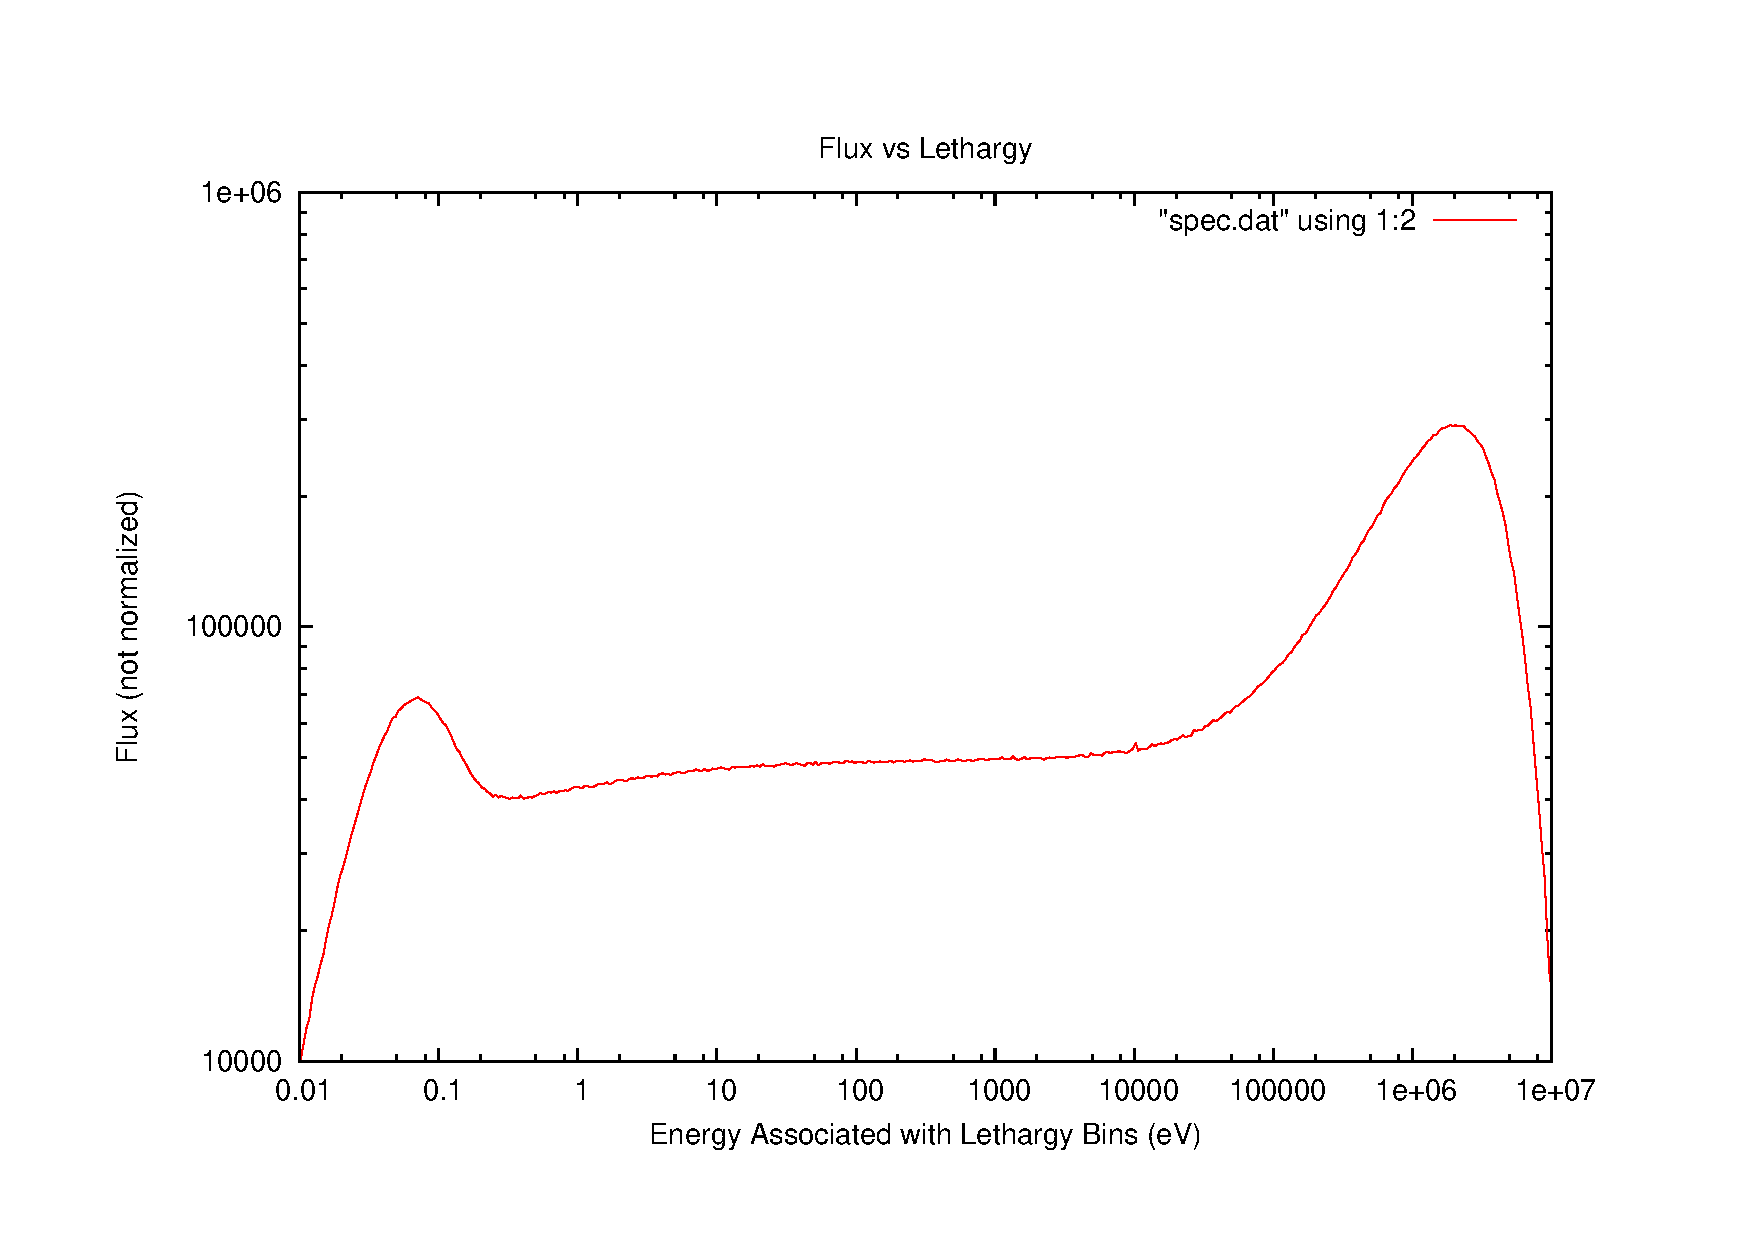
\includegraphics[width=4in]{images/spec.uncrop.pdf}
  \caption{Slowing Down with Maxwellian Free Gas Thermalization} \label{pset2}
\end{figure}


\end{document}
